\documentclass[serif]{beamer}
\usepackage[UTF8]{ctexcap}
\usepackage{amsmath,mathtools,hyperref,caption,wrapfig,enumerate,fontspec,mathrsfs,indentfirst,multicol}
\usetheme{Antibes}
\usecolortheme{beaver}

\newtheorem{thm}{定理}
\renewcommand\proofname{\heiti 证明}
\setlength{\parindent}{2em}

\usepackage{pgfplots}
\pgfplotsset{compat=1.15}
\usepackage{mathrsfs}

\setbeamerfont{title}{family=\heiti,series=\bfseries\selectfont}
\setbeamerfont{author}{family=\kaishu\selectfont}
\setbeamerfont{frametitle}{series=\bfseries\selectfont}
\setbeamerfont{framesubtitle}{family=\kaishu,series=\mdseries,shape=\itshape\selectfont}
\setbeamerfont{parttitle}{family=\heiti,series=\bfseries\selectfont}
\setbeamerfont{headline}{family=\fangsong,series=\bfseries\selectfont}

\setbeamertemplate{navigation symbols}{} 

\title{关于$\mathrm{e}$的不等式}
\author{程昊一}
\date{}


\begin{document}

\setlength\abovedisplayskip{0.2cm}
\setlength\belowdisplayskip{0.2cm}

\begin{frame}
	\maketitle
\end{frame}

\begin{frame}{目录}
	\begin{itemize}
		\item 实数与极限
		\item 自然底数$\mathrm{e}$
		\item 均值不等式
		\item $\mathrm{e}$与均值不等式的应用
	\end{itemize}
\end{frame}

\part{实数与极限}

\begin{frame}
	\partpage
	\noindent\begin{center}
		\kaishu 为了讲清楚什么是$\mathrm{e}$, 我们需要很多基本知识.
	\end{center}
\end{frame}

\begin{frame}{目录}
	\begin{multicols}{2}
		\tableofcontents
	\end{multicols}
\end{frame}

\section{\heiti 基础知识}
\subsection{\kaishu 基础数学与逻辑}

\begin{frame}{\S1 基础知识}{1.1 基础数学与逻辑}
	\noindent\textbf{1.}\par
	$\forall$表示“对于所有的”, 或者“对于每一个”; $\exists$表示“存在”, $\mathrm{s.t.}$表示“使得”. 例如: \par
	\begin{quotation}
		$\forall$整数$a$, $\exists$整数$b$, $\mathrm{s.t.}b>a$.
	\end{quotation}
	注意, 此命题与以下命题含义完全不同: 
	\begin{quotation}
		$\exists$整数$b$, $\mathrm{s.t.}\forall$整数$a$, $b>a$.
	\end{quotation}
	\noindent\textbf{2.}\par
	求和符号($\sum_{i=1}^n$). 例如:
	\[\sum\limits_{i=1}^{n}2i=n(n+1).\]
\end{frame}

\begin{frame}
	\noindent\textbf{3.}\par
	自然数集记为$\mathbb{N}$, 整数集记为$\mathbb{Z}$, 有理数集记为$\mathbb{Q}$, 实数集记为$\mathbb{R}$.\\
	\noindent\textbf{4.}\par
	符号$\Rightarrow$表示“蕴含着”, 符号$\Leftrightarrow$表示“等价于”或“当且仅当”. 例如:
	\begin{quotation}
		$n$为偶数$\Rightarrow n$为整数.\\
		$n$为偶数$\Leftrightarrow n$能被$2$整除.
	\end{quotation}
	\noindent\textbf{5.}\par
	一个命题可以记为$\mathbf{A}\Rightarrow\mathbf{B}$. 那么其逆命题为$\mathbf{B}\Rightarrow\mathbf{A}$, 否命题为$\neg\mathbf{A}\Rightarrow\neg\mathbf{B}$,
	逆否命题为$\neg\mathbf{B}\Rightarrow\neg\mathbf{A}$.\\
	一个命题与它的逆否命题等价. 即:
	\[(\mathbf{A}\Rightarrow\mathbf{B})\Leftrightarrow(\neg\mathbf{B}\Rightarrow\neg\mathbf{A}).\]\par
	\noindent\textbf{6.}\par
	符号$\wedge$表示“与”“并且”, 符号$\vee$表示“或”.
\end{frame}

\subsection{\kaishu 集合论}

\begin{frame}{1.2 集合论}
	\noindent\textbf{1.}\par
	\textbf{集合}是一堆\textbf{元素}的集体, 分为有限集与无限集. 没有元素的集合称为空集, 用$\varnothing$表示. 用$a\in A$表示元素$a$属于集合$A$.\par
	\noindent\textbf{2.}\par
	若每一个$i\in I$都对应一个集合$A_i$, 那么$\mathcal{A}=\{A_i\mid i\in I\}$就是\textbf{索引集}为$I$的集合$A$的\textbf{索引族}. 有时亦可记为$\{A_\alpha\}$.\par
	\noindent\textbf{3.}\par
	若集合$A$中的每一个元素同时是集合$B$的元素, 那么称$A$为$B$的\textbf{子集}, 记作$A\subseteq B$. 即:
	\[\forall x\in A(x\in B)\Leftrightarrow A\subseteq B.\]
	对于$\forall A$, $\varnothing\in A$.
\end{frame}

\begin{frame}
	\noindent\textbf{4.}\par
	开区间$(a,b)$定义为
	\[(a,b)=\{x\in\mathbb{R}\mid a<x<b\},\]
	闭区间$[a,b]$定义为
	\[[a,b]=\{x\in\mathbb{R}\mid a\le x\le b\},\]
	半开区间$(a,b]$或$[a,b)$定义为
	\[(a,b]=\{x\in\mathbb{R}\mid a<x\le b\},\]
	\[[a,b)=\{x\in\mathbb{R}\mid a\le x<b\}.\]
	
\end{frame}

\begin{frame}
	\noindent\textbf{5.}\par
	记$A$与$B$的元素共同构成的集合为$A$与$B$的并集, 记为$A\cup B$. 即:
	\[A\cup B=\{x\mid x\in A\vee x\in B\}.\]\par
	记既包含在$A$中又包含在$B$中的元素构成的集合为$A$与$B$的交集, 记为$A\cap B$. 即:
	\[A\cap B=\{x\mid x\in A\wedge x\in B\}.\]
	特别地, 若$A\cap B=\varnothing$, 则称$A$与$B$不相交.
\end{frame}

\section{\heiti 有理数的缺陷}
\subsection{\kaishu 整数与有理数的定义}

\begin{frame}{\S2 有理数的缺陷}{2.1 整数与有理数的定义}
	自然数由人们在生产劳动中抽象而来. 那么自然数的严格定义是什么?\par
	自然数的定义由\textbf{皮亚诺(Peano)公理}给出:\par
	\textbf{Peano公理}\quad\kaishu{设$\mathbb{N}$为一个非空集合, 满足下列条件:
	\begin{enumerate}
		\item 每一个$n\in\mathbb{N}$, 有唯一的一个$\mathbb{N}$中的元素与之对应, 称为$n$的{\heiti 后继元素}(或{\heiti 后继}), 记为$n^+$;
		\item 存在一个元素$e\in\mathbb{N}$, 它不是$\mathbb{N}$中任意一个元素的后继;
		\item $\mathbb{N}$中的元素至多是一个元素的后继, 即$a^+=b^+\Rightarrow a=b$;
		\item (归纳公理)设$S$为$\mathbb{N}$的一个非空子集, 且$e\in S$. 如果$n\in S\Rightarrow n^+\in S$, 则$S=\mathbb{N}$.
	\end{enumerate}
	那么, 这样的集合$\mathbb{N}$称为{\heiti 自然数集}, 它的元素称为{\heiti 自然数}.}
\end{frame}

\begin{frame}
	有了自然数, 我们就可以定义加法.\par
	\textbf{加法}\quad{\kaishu 在$\mathbb{N}$上存在且仅存在一个二元运算$\sigma$, 满足$\forall m,n\in\mathbb{N}$, 有:
	\begin{enumerate}
		\item $\sigma(n,e)=n^+$;
		\item $\sigma(n,m^+)=(\sigma(n,m))^+$.
	\end{enumerate}
	这样的二元运算称为{\heiti 加法}.}\par
	同样可以定义乘法:\par
	\textbf{乘法}\quad{\kaishu
	在$\mathbb{N}$上存在且仅存在一个二元运算$\pi$, 满足$\forall m,n\in\mathbb{N}$, 有:
	\begin{enumerate}
		\item $\pi(n,e)=n$;
		\item $\pi(n,m^+)=\pi(n,m)+n$.
	\end{enumerate}
	这样的二元运算称为{\heiti 乘法}.}\par
	证明从略. 
\end{frame}

\begin{frame}
	我们还可以继续定义负整数与整数, 及其加法与乘法, 但限于篇幅不再赘述.\par
	下面我们定义\textbf{有理数}:\par
	\textbf{有理数}\quad{\kaishu 定义$\mathbb{Q}=\{(p,q)\mid p,q\in\mathbb{Z}\wedge q\neq0\}$, 满足$\forall k,p,q,r,s\in\mathbb{Z}$, 有:
	\begin{enumerate}
		\item $(p,q)=(kp,kq)$;
		\item $(p,k)+(r,k)=(p+r,k)$;
		\item $(p,q)\cdot(r,s)=(pr,qs)$.
	\end{enumerate}
	}
	这其实和我们熟知的有理数是一致的, 并且容易验证由这三个运算的定义可以推出其他熟知的运算性质, 略.
\end{frame}

\subsection{\kaishu 上界与上确界}

\begin{frame}{2.2 上界与上确界}
	我们先来定义\textbf{有序集}:\par
	\textbf{有序集}\quad {\kaishu 集合$S$上的\textbf{顺序}是一种关系, 记作“$<$”, 满足:
	\begin{enumerate}
		\item $\forall x,y\in S$, $x<y$, $x=y$, $y<x$有且仅有一个成立;
		\item $\forall x,y\in S$, ($x<y\wedge y<z$)$\Rightarrow x<z$.
	\end{enumerate}
	}\par
	$x<y$也可以写作$y>x$, $x\le y$意为“$x<y$或$x=y$”. 由此可得:
	\[x\le y\Leftrightarrow\neg(x>y), x\ge y\Leftrightarrow\neg(x<y).\]
\end{frame}

\begin{frame}
	由此可以定义上、下界:\par
	\textbf{上界与下界}\quad{\kaishu 设$E$为有序集$S$的子集, 如果存在$\alpha\in S$, 使得$\forall x\in E$$(x\le\alpha)$, 那么称$\alpha$为$E$的\textbf{上界}.\par
	类似地, 如果$\exists\beta\in S$, 使得$\forall x\in E$$(x\ge\beta)$, 那么称$\beta$为$E$的\textbf{下界}.}\par
	注意, 一个集合的上界与下界并不一定是这个集合的元素.
\end{frame}

\begin{frame}
	我们还可以定义上确界与下确界:\par
	\textbf{上确界与下确界}\quad{\kaishu 设$E$为有序集$S$的子集. 如果$S$中存在$E$的一个上界$\alpha$, 使得任意一个$S$中小于$\alpha$的元素都不是$E$的上界, 那么$\alpha$为$E$的\textbf{最小上界}或\textbf{上确界}, 记为$\sup E$. 即:
	\begin{align*}
		\alpha=\sup E\Leftrightarrow&(\forall x\in E(x\le\alpha))\\
		\wedge&(\forall\gamma\in S\wedge\gamma<\alpha(\exists x\in E, \mathrm{s.t.}\gamma<x)).
	\end{align*}\par
	类似地, 如果$S$中存在$E$的一个下界$\beta$, 使得任意一个$S$中大于$\beta$的元素都不是$E$的下界, 那么$\beta$为$E$的\textbf{最大下界}或\textbf{下确界}, 记为$\inf E$. 即:
	\begin{align*}
		\beta=\inf E\Leftrightarrow&(\forall x\in E(x\ge\beta))\\
		\wedge&(\forall\gamma\in S\wedge\gamma>\beta(\exists x\in E, \mathrm{s.t.}\gamma>x)).
	\end{align*}
	}
\end{frame}

\subsection{\kaishu 有理数的缺陷}

\begin{frame}{2.3 有理数的缺陷}
	有理数的缺陷在哪里呢? 下面, 我们重点考察一个集合: $A=\{x\mid x\in\mathbb{Q}\wedge x^2<2\}$. 设全集$S=\mathbb{Q}$.\par
	\textbf{1. $E$有上界. }显然, 满足$x>0\wedge x\in\mathbb{Q}\wedge x^2>2$的数都为$A$的上界.\par
	\textbf{2. $E$没有上确界. }假设$E$有上确界, 设$\sup E=p\in\mathbb{Q}$.\par
	若$p^2<2$, 则令
	\[q=\frac{2p+2}{p+2},\]
	容易证明$p^2<q^2<2$, 且$q\in E$, 与上确界的定义矛盾.\par
	若$p^2>2$, 则$p^2>q^2>2$, 且$q$为$E$的上界, 与上确界的定义矛盾.\par
	所以无论$p$的值如何都会引发矛盾, 所以$E$不存在上确界.
\end{frame}

\begin{frame}
	也就是说, \textbf{有理数集的一个有上界的子集不一定有上确界. }这就是我们要将有理数扩充为实数的一个重要原因.
\end{frame}

\section{\heiti 实数的最小上界性}
\subsection{\kaishu 域}

\begin{frame}{\S3 实数的最小上界性}{3.1 域}
	我们先给出\textbf{域}的定义:\par
	\textbf{域}\quad{\kaishu 
	$F$是一个域, 当且仅当$F$是任意一个具有“加法”与“乘法”两种二元运算的集合, 且满足下列性质:\par
	\textbf{A1. }(加法的封闭性)$\forall x, y\in F(x+y\in F)$.\par
	\textbf{A2. }(加法交换律)$\forall x, y\in F(x+y=y+x)$.\par
	\textbf{A3. }(加法结合律)$\forall x, y, z\in F((x+y)+z=(y+x)+z)$.\par
	\textbf{A4. }(加法单位元)$\exists 0\in F$, $\mathrm{s.t. }\forall x\in F(x+0=x)$.\par
	\textbf{A5. }(加法的逆元)$\forall x\in F(\exists -x\in F, $$\mathrm{s.t. }x+(-x)=0)$.\par
	\textbf{M1. }(乘法的封闭性)$\forall x, y\in F(xy\in F)$.\par
	\textbf{M2. }(乘法交换律)$\forall x, y\in F(xy=yx)$.\par
	\textbf{M3. }(乘法结合律)$\forall x, y, z\in F((xy)z=x(yz))$.\par
	\textbf{M4. }(乘法单位元)$\exists 1\in F\wedge 1\neq 0, $$\mathrm{s.t }\forall x\in F(1\cdot x=x)$.\par
	\textbf{M5. }(乘法的逆元)$\forall x\in F(\exists x^{-1}\in F, $$\mathrm{s.t. }x(x^{-1})=1.)$\par
	\textbf{D. }(乘法对于加法的分配律)$\forall x, y, z\in F(x(y+z)=xy+xz)$.
	}
\end{frame}

\begin{frame}
	接着是\textbf{有序域}:\par
	\textbf{有序域}\quad {\kaishu 
	$F$是一个有序域, 当且仅当$F$是一个\textbf{有序集}, 并且$F$和两个二元运算构成\textbf{域}, 且满足下列公理:\par
	\textbf{O1. }如果$x,y\in F$且$x<y$, 那么$\forall z\in F(x+z<y+z)$.\par
	\textbf{O2. }如果$x,y\in F$且$x>0$, $y>0$, 那么$xy>0$.
	}
\end{frame}

\subsection{\kaishu 实数域的定义}

\begin{frame}{3.2 实数域的定义}
	我们可以正式地定义\textbf{实数}, 即\textbf{具有最小上界性且包含$\mathbb{Q}$的有序域}.\par 
	应当强调的是, 我们只是定义了$\mathbb{R}$, 但它不一定存在. 许多教科书假定了$\mathbb{R}$的存在性, 并称为\textbf{完备性公理}, 这里的“完备性”就是最小上界性与最大下界性的另一种说法. 不过, 在假设了$\mathbb{Q}$的存在性之后, 有一种(相当麻烦的)称为“戴德金(Dedekind)分割”的方法可以证明$\mathbb{R}$的存在性. 限于篇幅, 相关资料请自行查阅.
\end{frame}

\section{\heiti 序列极限}
\subsection{\kaishu 序列的定义}

\begin{frame}{\S4 序列极限}{4.1 序列的定义}
	实数集$\mathbb{R}$中的一个\textbf{序列}就是一个函数:
	\[f:\mathbb{N}\rightarrow\mathbb{R}, f: n\mapsto p_n,\]
	其中$p_n\in\mathbb{R}$. 我们通常把序列表示为$\{p_n\}$.如果
	\[\exists q,d\in R\wedge d>0, \mathrm{s.t.}\forall n\in\mathbb{N}_+(|p_n-q|<d),\]
	那么称$\{p_n\}$是\textbf{有界的}.
\end{frame}

\subsection{\kaishu 收敛与序列极限}

\begin{frame}{4.2 收敛与序列极限}
	设$\{p_n\}$为$\mathbb{R}$中的任意一个序列. 若$\forall\varepsilon>0$, $\exists N\in\mathbb{N}$, $\mathrm{s.t. }\forall n\ge N$$(|p_n-p|<\varepsilon)$, 那么称$p$为$\{p_n\}$的\textbf{极限}, 记为
	\[\lim\limits_{n\to\infty}p_n=p.\]
	或$p_n\to p$.
	\begin{figure}[htbp]
		\centering
		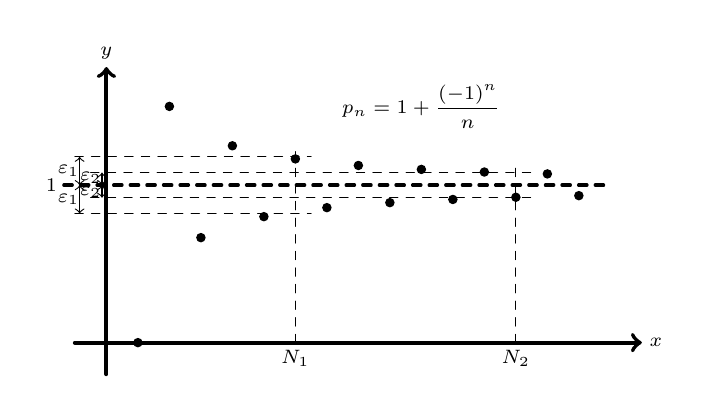
\begin{tikzpicture}[line cap=round,line join=round,x=0.4cm,y=2cm]
			\clip(-2.5,-0.3) rectangle (18,2);
			\draw [line width=0.4pt,dash pattern=on 3pt off 3pt] (-1.,0.82)-- (6.5,0.82);
			\draw [line width=0.4pt,dash pattern=on 3pt off 3pt] (-1.,1.18)-- (6.5,1.18);
			\draw [line width=0.4pt,dash pattern=on 3pt off 3pt] (-0.5,0.92)-- (13.5,0.92);
			\draw [line width=0.4pt,dash pattern=on 3pt off 3pt] (-0.5,1.08)-- (13.5,1.08);
			\draw [line width=1.2pt,dash pattern=on 3pt off 3pt] (-1.35,1.)-- (16.,1.);
			\draw [line width=0.4pt,dash pattern=on 3pt off 3pt] (6.,0.)-- (6.,1.23);
			\draw [line width=0.4pt,dash pattern=on 3pt off 3pt] (13.,0.)-- (13.,1.13);
			\draw [line width=0.4pt,<->] (-0.14,1.)-- (-0.14,1.08);
			\draw [line width=0.4pt,<->] (-0.14,1.)-- (-0.14,0.92);
			\draw [line width=0.4pt,<->] (-0.85,1.)-- (-0.85,1.18);
			\draw [line width=0.4pt,<->] (-0.85,1.)-- (-0.85,0.82);
			\draw [line width=1.5pt,->] (0.,-0.2)-- (0.,1.75);
			\draw [line width=1.5pt,->] (-1.,0.)-- (17.,0.);
			\begin{scriptsize}
				\draw [fill=black] (1.,0.) circle (1.5pt);
				\draw [fill=black] (2.,1.5) circle (1.5pt);
				\draw [fill=black] (3.,0.6666666666666667) circle (1.5pt);
				\draw [fill=black] (4.,1.25) circle (1.5pt);
				\draw [fill=black] (5.,0.8) circle (1.5pt);
				\draw [fill=black] (6.,1.1666666666666667) circle (1.5pt);
				\draw [fill=black] (7.,0.8571428571428572) circle (1.5pt);
				\draw [fill=black] (8.,1.125) circle (1.5pt);
				\draw [fill=black] (9.,0.8888888888888888) circle (1.5pt);
				\draw [fill=black] (10.,1.1) circle (1.5pt);
				\draw [fill=black] (11.,0.9090909090909091) circle (1.5pt);
				\draw [fill=black] (12.,1.0833333333333333) circle (1.5pt);
				\draw [fill=black] (13.,0.9230769230769231) circle (1.5pt);
				\draw [fill=black] (14.,1.0714285714285714) circle (1.5pt);
				\draw [fill=black] (15.,0.9333333333333333) circle (1.5pt);
				\node at (-1.2,1.09) {$\varepsilon_1$};
				\node at (-1.2,0.91) {$\varepsilon_1$};
				\node at (-0.5,1.045) {$\varepsilon_2$};
				\node at (-0.5,0.955) {$\varepsilon_2$};
				\node at (-1.75,1) {1};
				\node at (0.,1.75) [above] {$y$};
				\node at (17.,0.) [right] {$x$};
				\node at (6,0) [below] {$N_1$};
				\node at (13,0) [below] {$N_2$};
				\node at (10,1.5) {$\displaystyle p_n=1+\frac{(-1)^n}{n}$};
			\end{scriptsize}
		\end{tikzpicture}
	\end{figure}
\end{frame}

\section{\heiti 单调有界序列的极限}
\subsection{\kaishu 单调序列}

\begin{frame}{\S5 单调有序数列的极限}{5.1 单调序列}
	单调序列, 即只增不减或只减不增的序列, 严格表述即: \par
	\textbf{单调序列}\quad {\kaishu 设$\{p_n\}$为$\mathbb{R}$中的任意一个序列. 若$\forall n\in\mathbb{N}$$(p_n\le p_{n+1})$, 那么$\{p_n\}$是\textbf{单调递增}的; 若$\forall n\in\mathbb{N}$$(p_n\ge p_{n+1})$, 那么$\{p_n\}$是\textbf{单调递减}的. }
\end{frame}

\subsection{\kaishu 单调有界序列的极限}

\begin{frame}{5.2 单调有界序列的极限}
	我们将给出$\mathbb{R}$非常重要的一个性质: \textbf{$\mathbb{R}$中的单调有界序列必有极限.}
	即:\par
	若$\mathbb{R}$中的序列$\{p_n\}$为单调有界序列, 那么极限
	\[\lim\limits_{n\to\infty}p_n\]
	存在.\par
	我们将给出证明:
\end{frame}

\begin{frame}
	不妨设$\{p_n\}$为单调递增的. 设
	\[P=\{p_k\mid k\in\mathbb{N}_+\},\]
	则$P\in\mathbb{R}$. 那么由实数的最小上界性可知$\sup P$存在, 记为$\alpha$.\par
	对$\forall\varepsilon>0$, 设\[\beta=\alpha-\varepsilon, \]
	则由上确界的定义可知, $\exists p_N\in P$, 使得$p_N>\beta.$\par
	又由于$\{p_n\}$是单调递增的, 所以$\forall k>N$, 有$p_k>\beta$.\par
	即,
	\[\forall\varepsilon>0, \exists N\in\mathbb{N}_+, \text{ s.t. }(\forall k>N\wedge k\in\mathbb{N}_+(p_k<|\alpha-p_N|)).\]
	\begin{figure}[htbp]
		\centering
		\begin{tikzpicture}[line cap=round,line join=round,x=1.8cm,y=1.8cm]
			\clip(-0.5,-1.) rectangle (5.5,0.5);
			\draw [line width=1.2pt,->] (0.,0.)-- (5.,0.);
			\draw [line width=0.4pt,<->] (3.,0.25)-- (4.,0.25);
			\draw [line width=0.4pt,dash pattern=on 1pt off 1pt] (3.,0.)-- (3.,0.35);
			\draw [line width=0.4pt,dash pattern=on 1pt off 1pt] (4.,0.)-- (4.,0.35);
			\draw [fill=black] (1.,0.) circle (1.5pt);
			\draw[color=black] (1.013611751296384,-0.2) node {$p_1$};
			\draw [fill=black] (1.5,0.) circle (1.5pt);
			\draw[color=black] (1.4941668332076354,-0.2) node {$p_2$};
			\draw [fill=black] (1.8,0.) circle (1.5pt);
			\draw[color=black] (1.859032728732845,-0.2) node {$p_3$};
			\draw [fill=black] (4.,0.) circle (2.0pt);
			\draw[color=black] (4,-0.4) node {$\alpha$};
			\draw [fill=black] (3.,0.) circle (2.0pt);
			\draw[color=black] (3,-0.4) node {$\beta$};
			\draw[color=black] (3.5,0.4515800012625302) node {$\varepsilon$};
			\draw [fill=black] (3.25,0.) circle (1.5pt);
			\draw[color=black] (3.256202133548891,-0.2) node {$p_N$};
			\draw [fill=black] (2.75,0.) circle (1.5pt);
			\draw[color=black] (2.722252042536389,-0.2) node {$p_{N-1}$};
			\node at (2.25,-0.175) {...};
		\end{tikzpicture}
	\end{figure}
\end{frame}

\part{自然底数$\mathrm{e}$}

\begin{frame}
	\partpage
	\noindent\begin{center}
		\kaishu 我们终于搞懂了什么是实数! 于是便可以定义自然底数$\mathrm{e}$并探究其性质.
	\end{center}
\end{frame}
  
\begin{frame}{目录}
	\tableofcontents
\end{frame}

\section{\heiti 定义与概述}

\begin{frame}{\S1 定义与概述}
	自然底数$\mathrm{e}$被定义为
	\[\lim\limits_{n\to\infty}\left(1+\frac{1}{n}\right)^n.\]
	即, $\mathrm{e}$就是数列$\{(1+1/n)^n\}$的极限.\par
	但是我们还没有说明$\mathrm{e}$的存在性. 下面我们将说明$\{p_n\}$$=\{(1+1/n)^n\}$是一个单调递增的有界数列.
\end{frame}

\begin{frame}
	\textbf{1. $\{p_n\}$单调递增}\par
	对$p_n$与$p_{n+1}$进行二项式展开:
	\begin{align*}
		\left(1+\frac{1}{n}\right)^n&=\sum\limits_{i=0}^n{\mathrm{C}_n^i\cdot\frac{1}{n^i}}=\sum\limits_{i=0}^n{\frac{n!}{i!(n-i)!}\cdot\frac{1}{n^i}}\\
		&=\sum\limits_{i=0}^n{\frac{1}{i!}\cdot\left[\frac{n}{n}\cdot\frac{n-1}{n}\cdots\frac{n-(i-1)}{n}\right]}\\
		&=1+1+\sum\limits_{i=2}^n{\frac{1}{i!}\left(1-\frac{1}{n}\right)\left(1-\frac{2}{n}\right)\cdots\left(1-\frac{i-1}{n}\right)};\\
		\left(1+\frac{1}{n+1}\right)^{n+1}&=1+1+\sum\limits_{i=2}^n\left[\frac{1}{i!}\left(1-\frac{1}{n+1}\right)\left(1-\frac{2}{n+1}\right)\right.\\
		&\left.\cdots\left(1-\frac{i-1}{n+1}\right)\right]+\frac{1}{(n+1)^{n+1}}.
	\end{align*}
\end{frame}

\begin{frame}
	对比求和符号中的式子, 发现后者总是比前者大, 所以我们可以得到
	\[\left(1+\frac{1}{n}\right)^n<\left(1+\frac{1}{n+1}\right)^{n+1}.\]\par
\end{frame}

\begin{frame}
	\textbf{2. $\{p_n\}$有界}\par
	我们可以证明$\forall n\in\mathbb{N}_+(p_n<3)$.事实上,
	\begin{align*}
		\left(1+\frac{1}{n}\right)^n&=1+1+\sum\limits_{i=2}^n{\frac{1}{i!}\left(1-\frac{1}{n}\right)\left(1-\frac{2}{n}\right)\cdots\left(1-\frac{i-1}{n}\right)}\\
		&<1+1+\sum\limits_{i=2}^n{\frac{1}{i!}}\\
		&<1+1+\sum\limits_{i=2}^n\frac{1}{(i-1)i}\\
		&=3-\frac{1}{n}<3.
	\end{align*}
	综上, 我们就证明了$\{p_n\}$是一个单调递增的有界数列.
\end{frame}

\begin{frame}
	那么, 我们就说明了$\mathrm{e}=\lim\limits_{n\to\infty}(1+1/n)^n$的存在性.\par
	为什么说$\mathrm{e}$是自然底数? 这就不得不提及$\mathrm{e}$的“自然”之处. 事实上, 自然中充满了“变化速度与自身的量成正比”的变化过程. 例如, 一杯开水放在常温的房间内, 温度变低的速度就与杯中水的温度与室温的差成正比. 再比如, 一个弹簧一端连接墙, 另一端挂一个重物, 重物受到一个与自身速度成正比且反向的阻力, 那么重物的振幅的衰减也满足上述规律(即“变化速度与自身的量成正比”). 自然中有许多类似的变化过程, 都符合这条规律.\par
	如果学过常微分方程, 那么上述的函数都是方程
	\[y'=\alpha y\]
	的解, 其解即为
	\[y=k\mathrm{e}^{\alpha x}.\]
\end{frame}

\section{\heiti 关于$\mathrm{e}$的不等式}
\subsection{\kaishu 两个不同的序列}

\begin{frame}{\S2 关于$\mathrm{e}$的不等式}{2.1 两个不同的序列}
	我们重点考察两个序列:
	\[\{p_n\}=\left\{\left(1+\frac{1}{n}\right)^n\right\}; \{q_n\}=\left\{\left(1+\frac{1}{n}\right)^{n+1}\right\}.\]\par
	我们已经了解了$\{p_n\}$: 单调有界的递增序列, 其极限为$\mathrm{e}$. 我们仍然可以用相同的方式考察$\{q_n\}$.
\end{frame}

\begin{frame}
	首先, $\{q_n\}$是递减的. 我们采用另一种方法证明. 首先我们先证明一个不等式: 对于$b>a>0$与$n\in\mathbb{N}_+$, 有
	\[b^{n+1}>\left[(n+1)(b-a)+a\right]a^n.\]\par
	事实上, 
	\begin{align*}
		b^{n+1}-a^{n+1}&=(b-a)\left(b^n+b^{n-1}a+b^{n-2}a^2+\cdots+a^n\right)\\
		&>(b-a)\cdot(n+1)a^n.
	\end{align*}
	整理, 得
	\begin{align*}
		b^{n+1}&>a^{n+1}+(b-a)(n+1)a^n\\
		&=\left[(n+1)(b-a)+a\right]a^n.
	\end{align*}
\end{frame}

\begin{frame}
	那么, 令$b=1+1/n$, $a=1+1/(n+1)$, 可得
	\begin{align*}
		\left(1+\frac{1}{n}\right)^{n+1}&>\left[(n+1)\left(\frac{1}{n}-\frac{1}{n+1}\right)+1+\frac{1}{n+1}\right]\left(1+\frac{1}{n+1}\right)^n\\
		&=\left(1+\frac{1}{n}+\frac{1}{n+1}\right)\left(1+\frac{1}{n+1}\right)^n\\
		&=\left[1+\frac{2}{n+1}+\left(\frac{1}{n}-\frac{1}{n+1}\right)\right]\left(1+\frac{1}{n+1}\right)^n\\
		&>\left[1+\frac{2}{n+1}+\left(\frac{1}{n+1}\right)^2\right]\left(1+\frac{1}{n+1}\right)^n\\
		&=\left(1+\frac{1}{n+1}\right)^2\left(1+\frac{1}{n+1}\right)^n=\left(1+\frac{1}{n+1}\right)^{n+2}.
	\end{align*}
\end{frame}

\begin{frame}
	而且, 
	\[\lim\limits_{n\to\infty}q_n=\left[\lim\limits_{n\to\infty}\left(1+\frac{1}{n}\right)^n\right]\left[\lim\limits_{n\to\infty}\left(1+\frac{1}{n}\right)\right]=\lim\limits_{n\to\infty}\left(1+\frac{1}{n}\right)^n=\mathrm{e}.\]
	所以我们可以看到, $\{p_n\}$从负方向趋近于$\mathrm{e}$, 而$\{q_n\}$从正方向趋近于$\mathrm{e}$.
	\begin{figure}[htbp]
		\centering
		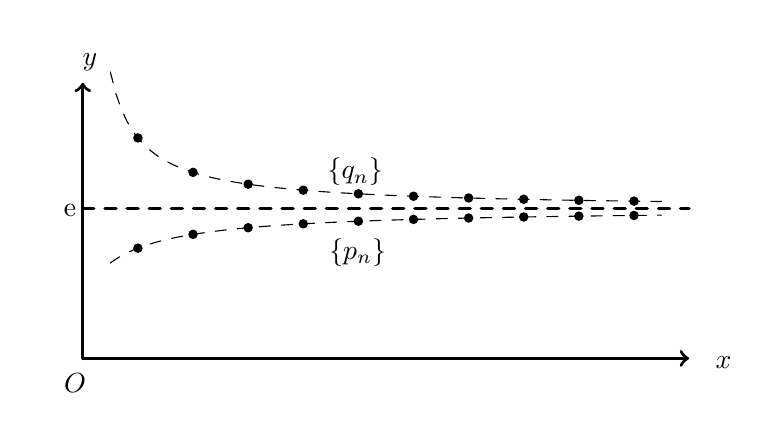
\begin{tikzpicture}[line cap=round,line join=round,x=0.7cm,y=0.7cm]
			\clip(-1.,-1.) rectangle (12.,6.);
			\draw [line width=1.2pt,->] (0.,0.)-- (11.,0.);
			\draw [line width=1.2pt,->] (0.,0.)-- (0.,5.);
			\draw [line width=0.4pt,dash pattern=on 4pt off 4pt,domain=0.5:10.5,samples=100] plot(\x,{(1+1/\x)^\x});
			\draw [line width=0.4pt,dash pattern=on 4pt off 4pt,domain=0.5:10.5,samples=100] plot(\x,{(1+1/\x)^(\x+1)});
			\draw [line width=1.2pt,dash pattern=on 4pt off 4pt] (0.,2.718281828459045)-- (11.,2.718281828459045);
			\draw (4.295221038657742,2.348763954116683) node[anchor=north west] {$\{p_n\}$};
			\draw (4.265395544763088,3.8102131549547265) node[anchor=north west] {$\{q_n\}$};
			\draw (-0.51720699669759115,-0.0969391650703095) node[anchor=north west] {$O$};
			\draw (11.304212103901433,0.2055431162275411) node[anchor=north west] {$x$};
			\draw (-0.17877755164570508,5.704132017265253) node[anchor=north west] {$y$};
			\draw (-0.5215962253288802,2.964575807588378) node[anchor=north west] {$\mathrm{e}$};
			\draw [fill=black] (1.,2.) circle (1.5pt);
			\draw [fill=black] (2.,2.25) circle (1.5pt);
			\draw [fill=black] (3.,2.37037037037037) circle (1.5pt);
			\draw [fill=black] (4.,2.44140625) circle (1.5pt);
			\draw [fill=black] (5.,2.48832) circle (1.5pt);
			\draw [fill=black] (6.,2.5216263717421135) circle (1.5pt);
			\draw [fill=black] (7.,2.546499697040712) circle (1.5pt);
			\draw [fill=black] (8.,2.565784513950348) circle (1.5pt);
			\draw [fill=black] (9.,2.5811747917131984) circle (1.5pt);
			\draw [fill=black] (10.,2.5937424601000023) circle (1.5pt);
			\draw [fill=black] (1.,4.) circle (1.5pt);
			\draw [fill=black] (2.,3.375) circle (1.5pt);
			\draw [fill=black] (3.,3.160493827160493) circle (1.5pt);
			\draw [fill=black] (4.,3.0517578125) circle (1.5pt);
			\draw [fill=black] (5.,2.9859839999999993) circle (1.5pt);
			\draw [fill=black] (6.,2.9418974336991326) circle (1.5pt);
			\draw [fill=black] (7.,2.910285368046528) circle (1.5pt);
			\draw [fill=black] (8.,2.8865075781941414) circle (1.5pt);
			\draw [fill=black] (9.,2.8679719907924426) circle (1.5pt);
			\draw [fill=black] (10.,2.8531167061100025) circle (1.5pt);
		\end{tikzpicture}
	\end{figure}
\end{frame}

\subsection{\kaishu $\mathrm{e}$与调和级数}

\begin{frame}{2.2 $\mathrm{e}$与调和级数}
	所谓调和级数, 就是指
	\[H(n)=\sum\limits_{i=1}^n{\frac{1}{i}}.\]\par
	我们在此先给出结论: 对于任意的$n\in\mathbb{N}_+$, 有
	\[H(n)>\ln{n};\]
	并且极限
	\[\gamma=\lim\limits_{n\to\infty}[H(n)-\ln{n}]=0.577216\cdots\]
	存在, 被称为欧拉(Euler)常数.
\end{frame}

\begin{frame}
	事实上, 我们就是要证明数列
	\[\{a_n\}=\{H(n)-\ln{n}\}\]
	有一个确定的极限. 那么我们就即证$\{a_n\}$是一个单调递减的有界数列.\par
	首先, 我们有
	\[\left(1+\frac{1}{n}\right)^n<\mathrm{e}<\left(1+\frac{1}{n}\right)^{n+1},\]
	同时取自然对数并整理, 可得
	\[\frac{1}{n+1}<\ln{\frac{n+1}{n}}<\frac{1}{n}.\]\par
	这是一个很重要的不等式.
\end{frame}

\begin{frame}
	我们仍然分两步证明:\par
	\textbf{1. $\{a_n\}$单调递减}\par
	这是容易证明的, 因为$H(n)$与$H(n+1)$相减可以抵消大部分的项:
	\begin{align*}
		a_n-a_{n+1}&=\sum\limits_{i=1}^{n}{\frac{1}{i}}-\ln{n}-\sum\limits_{i=1}^{n+1}{\frac{1}{i}}+\ln{(n+1)}\\
		&=\ln{(n+1)}-\ln{n}-\frac{1}{n+1}\\
		&=\ln{\frac{n+1}{n}}-\frac{1}{n+1}>0.
	\end{align*}
	所以, 我们有
	\[a_n>a_{n+1}.\]
\end{frame}

\begin{frame}
	\textbf{2. $\{a_n\}$有界.}\par
	我们可以证明$\forall n\in\mathbb{N}_+(a_n>0)$. 事实上:
	\begin{align*}
		a_n&=\sum\limits_{i=1}^{n}{\frac{1}{i}}-\ln{n}>\sum\limits_{i=1}^{n}{\ln{\frac{1+i}{i}}}-\ln{n}\\
		&=\ln{\left(\frac{n+1}{n}\cdot\frac{n}{n-1}\cdots\frac{2}{1}\right)}-\ln{n}\\
		&=\ln{(n+1)}-\ln{n}>0.
	\end{align*}\par
	于是我们便证明了$\{a_n\}$是一个单调递减的有界数列. 那么极限
	\[\lim\limits_{n\to\infty}a_n\]
	便存在.
\end{frame}

\part{均值不等式}

\begin{frame}
	\partpage
	\noindent\begin{center}
		\kaishu 在了解完$\mathrm{e}$之后, 我们再来看一下另一个重要的不等式——均值不等式.
	\end{center}
\end{frame}

\begin{frame}{目录}
	\tableofcontents
\end{frame}

\section{\heiti 概述}

\begin{frame}{\S1 概述}
	首先我们了解一下平均值的本质.\par
	设有一组数$a_1$, $a_2$, $\cdots$, $a_n$与一种运算“$\ast$”. 若存在一个数$m$使得
	\[a_1\ast a_2\ast\cdots\ast a_n=m\ast m\ast\cdots\ast m,\]
	那么我们就可以称$m$为$a_i$($i=1,2,\cdots,n$)的平均值.
\end{frame}

\begin{frame}
	以下讨论均默认$a_i>0$($i=1,2,\cdots,n$).\par
	例如, 我们取“$\ast$”为“$+$”, 于是就有了算术平均数:
	\[A_n=\frac{1}{n}\sum\limits_{i=1}^n{a_i}; \]
	取“$\ast$”为“$\times$”, 就有了几何平均数:
	\[G_n=\sqrt[n]{a_1a_2\cdots a_n}.\]\par
	另外, 还有
	\[Q_n=\sqrt{\frac{1}{n}\sum\limits_{i=1}^n{a_i^2}}; H_n=\frac{n}{\sum\limits_{i=1}^n{\frac{1}{a_i}}},\]
	分别称为“平方平均数”“调和平均数”, 其中“$\ast$”分别取“平方后相加”和“取到数后相加”.
\end{frame}

\begin{frame}
	那么, 所谓均值不等式, 就是“算术平均值”$>$“几何平均值”. 即:\par 
	\textbf{均值不等式}\quad {\kaishu 设$a_i\ge0$($i=1,2,\cdots,n$), 则
	\[\frac{1}{n}\sum\limits_{i=1}^n{a_i}\ge\sqrt[n]{a_1a_2\cdots a_n}.\]
	等号等且仅当$a_1=a_2=\cdots=a_n$时取到.}
\end{frame}

\section{\heiti 证明选讲}
\subsection{\kaishu 调整法}

\begin{frame}{\S2 证明选讲}{2.1 调整法}
	我们将介绍一种证明不等式的强有力的方式——调整法.\par
	调整法的基本思路是: 设有一个代数式
	\[f\left(a_1,a_2,\cdots,a_n\right),\]
	如果我们想证明在$a_1=a_2=\cdots=a_n=A_n$的时候取到最大值, 那么可以采用如下办法:\par
	如果我们可以证明$\forall a_i\in\mathbb{R}$, $i=1,2,\cdots,n$, 有
	\[f\left(a_1,a_2,\cdots,a_n\right)\le f\left(A_n,a_1+a_2-A_n,\cdots,a_n\right)\]
	(即, 调整$n$个元中的某两项, 使得其中一个达到取等条件$A_n$, 两数和不变), 那么(不等号上方的数字为调整的元的位置):
\end{frame}

\begin{frame}
	\begin{align*}
		f\left(a_1,a_2,\cdots,a_n\right)&\overset{1}{\le}f\left(A_n,a_1+a_2-A_n,\cdots,a_n\right)\\
		&\overset{2}{\le}f\left(A_n,A_n,a_1+a_2+a_3-2A_n,\cdots,a_n\right)\\
		&\overset{3}{\le}f\left(A_n,A_n,A_n,\left(\sum\limits_{i=1}^4{a_i}\right)-3A_n,\cdots,a_n\right)\\
		&\overset{4}{\le}\cdots\\
		&\cdots\\
		&\overset{n}{\le}f\left(A_n,\cdots,A_n,\left(\sum\limits_{i=1}^n{a_i}\right)-(n-1)A_n\right)\\
		&=f\left(A_n,A_n,\cdots,A_n\right).
	\end{align*}\par
	这样, 就可以证明$\forall a_i\in\mathbb{R}$, $i=1,2,\cdots,n$, 有
	\[f\left(a_1,a_2,\cdots,a_n\right)\le f\left(A_n,A_n,\cdots,A_n\right).\]
\end{frame}

\begin{frame}
	下面我们就用调整法证明均值不等式.\par
	设对于$a_i\ge0$ ($i=1,2,\cdots,n$),
	\[f\left(a_1,a_2,\cdots,a_n\right)=a_1a_2\cdots a_n.\]
	我们知道在
	\[a_1=a_2=\cdots a_n=A_n\]
	时, $f$有最大值$A_n^n$. 那么我们可以通过证明: $\forall a_i\ge0$, $i=1,2,\cdots,n$, $a_1$为$a_i$中的最大值, $a_2$为$a_i$中的最小值, 那么
	\[f\left(a_1,a_2,\cdots,a_n\right)\le f\left(A_n,a_1+a_2-A_n,\cdots,a_n\right).\]
	我们在后面将会解释为什么要让$a_1$与$a_2$为最大值和最小值.
\end{frame}

\begin{frame}
	事实上,
	\begin{align*}
		&&f\left(a_1,a_2,\cdots,a_n\right)&\le f\left(A_n,a_1+a_2-A_n,\cdots,a_n\right)\\
		\Leftrightarrow&&a_1a_2a_3\cdots a_n&\le A_n(a_1+a_2-A_n)a_3\cdots a_n\\
		\overset{\small a_i\ge0}{\Leftrightarrow}&&a_1a_2&\le A_n(a_1+a_2-A_n)\\
		\Leftrightarrow&&A_n^2-A_na_1-A_na_2+a_1a_2&\le0\\
		\Leftrightarrow&&(A_n-a_1)(A_n-a_2)&\le0.
	\end{align*}
	因为$a_1$为$a_i$中的最大值, 且$a_2$为$a_i$中的最小值, 所以
	\[a_2\le A_n\le a_1.\]\par
	故上个不等式的最后一步成立. 于是我们就证明了调整一步后, $f$总是增大的.
\end{frame}

\begin{frame}
	于是, 对于一组不全相等的正实数$a_1,a_2,\cdots,a_n$, 我们可以进行调整以证明结论.\par
	首先, 因为$a_i$($i=1,2,\cdots,n$)不全相等, 所以必存在最大值与最小值. 由于每个元的地位都是等价的, 所以不妨设最大值为$a_1$, 最小值为$a_2$. 那么由上面的讨论, 我们有
	\[f\left(a_1,a_2,\cdots,a_n\right)\le f\left(A_n,a_1+a_2-A_n,a_3,\cdots,a_n\right).\]\par
	接下来我们考察括号中后$n-1$个数, 即$a_1+a_2-A_n$, $a_2$, $\cdots$, $a_n$. 容易知道, 这$n-1$个数的平均值仍然为$A_n$. 我们仍然可以找到最大值与最小值. 不妨设最大值为$a_1+a_2-A_n$, 最小值为$a_3$. 注意: $a_1+a_2-A_n$与其他元只是形式不一样, 但地位仍然是等价的, 所以我们仍然可以不妨设. 那么,
	\begin{small}
		\[f\left(A_n,a_1+a_2-A_n,\cdots,a_n\right)\le f\left(A_n,A_n,a_1+a_2+a_3-2A_n,\cdots,a_n\right).\]
	\end{small}
\end{frame}

\begin{frame}
	于是, 仿照上面的流程, 直到剩下的数均相等, 即均为$A_n$为止, 此时$f$的值为
	\[f\left(A_n,A_n,\cdots,A_n\right)=A_n^n.\]\par
	那么根据前面所说的, 我们就证明了$\forall a_i\ge0$, $i=1,2,\cdots,n$,
	\[f\left(a_1,a_2,\cdots,a_n\right)\le f\left(A_n,A_n,\cdots,A_n\right),\]
	即
	\[a_1a_2\cdots a_n\le A_n^n.\]
	又
	\[A_n^n=\left(\frac{1}{n}\sum\limits_{i=1}^n{a_i}\right)^n,\]
	所以
	\[\sqrt[n]{a_1a_2\cdots a_n}\le\frac{1}{n}\sum\limits_{i=1}^n{a_i}.\]
\end{frame}

\subsection{\kaishu 反向归纳法}

\begin{frame}{2.2 反向归纳法}
	我们用另一种方法证明均值不等式, 即所谓的反向归纳法.\par
	我们用$P(n)$表示$n$元均值不等式的命题. 那么我们可以通过证明下面三个命题以证明$\forall n\in\mathbb{N}_+$, $P(n)$均成立:{\kaishu
	\begin{enumerate}
		\item $P(2)$成立;
		\item $(P(n)\wedge P(2))\Rightarrow P(2n)$;
		\item $P(n)\Rightarrow P(n-1)$.
	\end{enumerate}
	}
	下面我们将分别给出证明.
\end{frame}

\begin{frame}
	\textbf{1. $P(2)$成立}\par
	事实上, $P(2)$即为
	\[\frac{a_1+a_2}{2}\ge\sqrt{a_1a_2}\Leftrightarrow\frac{1}{2}(\sqrt{a_1}-\sqrt{a_2})^2\ge0.\]
	这是显然成立的.\par
	\textbf{2. $(P(n)\wedge P(2))\Rightarrow P(2n)$}\par
	事实上,
	\begin{align*}
		\prod\limits_{i=1}^{2n}{a_i}&=\left(\prod\limits_{i=1}^{n}{a_i}\right)\left(\prod\limits_{i=n+1}^{2n}{a_i}\right)\overset{P(n)}{\le}\left(\sum\limits_{i=1}^{n}\frac{a_i}{n}\right)^n\left(\sum\limits_{i=n+1}^{2n}\frac{a_i}{n}\right)^n\\
		&\overset{P(2)}{\le}\left(\frac{1}{2}\sum\limits_{i=1}^{2n}\frac{a_i}{n}\right)^{2n}=\left(\sum\limits_{i=1}^{2n}\frac{a_i}{2n}\right)^{2n}.
	\end{align*}
	所以, 
	\[\sqrt[2n]{a_1a_2\cdots a_{2n}}\le\sum\limits_{i=1}^{2n}\frac{a_i}{2n}.\]
\end{frame}

\begin{frame}
	\textbf{3. $P(n)\Rightarrow P(n-1)$}\par
	令$A$为$a_1,a_2,\cdots,a_{n-1}$的平均值, 即$\sum_{i=1}^{n-1}a_i/(n-1)$. 那么,
	\[\left(\prod\limits_{i=1}^{n-1}a_i\right)A\overset{P(n)}{\le}\left[\frac{\left(\sum_{i=1}^{n-1}a_i\right)+A}{n}\right]^n=\left(\frac{(n-1)A+A}{n}\right)^n=A^n.\]
	所以, 
	\[\prod\limits_{i=1}^{n-1}a_i\le A^{n-1},\]
	即
	\[\sqrt[n-1]{a_1a_2\cdots a_{n-1}}\le\sum\limits_{i=1}^{n-1}\frac{a_i}{n-1}.\]\par
	综上, 我们证明了以上三个命题, 于是均值不等式得证.
\end{frame}


\part{$\mathrm{e}$与均值不等式的应用}

\begin{frame}
	\partpage
	\noindent\begin{center}
		\kaishu 接下来, 我们将应用$\mathrm{e}$与均值不等式, 来解决实际问题.
	\end{center}
\end{frame}

\begin{frame}{目录}
	\tableofcontents
\end{frame}

\section{\heiti 用均值不等式证明有关$\mathrm{e}$的不等式}

\begin{frame}{\S1 用均值不等式证明有关$\mathrm{e}$的不等式}
	我们证明的是以下两个数列:
	\[\{p_n\}=\left\{\left(1+\frac{1}{n}\right)^n\right\}; \{q_n\}=\left\{\left(1+\frac{1}{n}\right)^{n+1}\right\}\]
	分别单调递增与递减.
\end{frame}

\begin{frame}
	\textbf{1. $\{p_n\}$递增}\par
	为了方便起见, 设
	\[a_1=a_2=\cdots=a_n=1+\frac{1}{n}, a_{n+1}=1.\]
	那么由均值不等式, 有
	\[\frac{1}{n+1}\sum\limits_{i=1}^{n+1}a_i>\sqrt[n+1]{a_1a_2\cdots a_n}.\]\par
	而不等式左边为
	\[\frac{1}{n+1}\left[n\left(1+\frac{1}{n}\right)+1\right]=\frac{n+2}{n+1}=1+\frac{1}{n+1},\]
	不等式右边为
	\[\sqrt[n+1]{\left(1+\frac{1}{n}\right)^n}.\]
\end{frame}

\begin{frame}
	所以, 
	\[1+\frac{1}{n+1}>\sqrt[n+1]{\left(1+\frac{1}{n}\right)^n}.\]
	整理即得
	\[\left(1+\frac{1}{n}\right)^n<\left(1+\frac{1}{n+1}\right)^{n+1}.\]
	我们便证明了$p_n<p_{n+1}.$
\end{frame}

\begin{frame}
	\textbf{2. $\{q_n\}$递减}\par
	取
	\[b_1=\cdots=b_n=1-\frac{1}{n},b_{n+1}=1.\]
	由均值不等式, 有
	\[\frac{1}{n+1}\sum\limits_{i=1}^{n+1}b_i>\sqrt[n+1]{b_1b_2\cdots b_n}.\]\par
	而不等式左边为
	\[\frac{1}{n+1}\left[n\left(1-\frac{1}{n}\right)+1\right]=\frac{n}{n+1},\]
	不等式右边为
	\[\sqrt[n+1]{\left(\frac{n-1}{n}\right)^n}.\]
\end{frame}

\begin{frame}
	所以,
	\[\frac{n}{n+1}>\sqrt[n+1]{\left(\frac{n-1}{n}\right)^n}.\]
	化简即得
	\[\left(1+\frac{1}{n}\right)^{n+1}<\left(1+\frac{1}{n-1}\right)^n.\]\par
	我们便证明了$q_n>q_{n+1}.$
\end{frame}

\section{\heiti 正数的拆分}

\begin{frame}{\S2 正数的拆分}
	这一节我们主要讨论课本上的问题:\par
	{\kaishu 将正数$s$拆分若干个正数$a_1$, $a_2$, $\cdots$, $a_n$, 使它们的乘积最大. }\par
	首先, 在变量的个数$n$确定的情况下, 
	\[a_1a_2\cdots a_n\le\left(\frac{1}{n}\sum\limits_{i=1}^{n}a_i\right)^n=\left(\frac{s}{n}\right)^n.\]
	那么我们就重点研究
	\[\{p_n\}=\left\{\left(\frac{s}{n}\right)^n\right\}\]
	的最大值.
\end{frame}

\begin{frame}
	类似于“差分”的思想, 我们可以将此数列相邻两项做商, 通过比较这个商与$1$的大小从而判断哪一项更大. \par
	记
	\[k_n=\frac{p_n}{p_{n+1}}.\]
	那么
	\begin{align*}
		k_n&=\left(\frac{s}{n}\right)^n\left/\left(\frac{s}{n+1}\right)^{n+1}\right.\\
		&=\frac{s^n(n+1)^{n+1}}{s^{n+1}n^n}=\frac{(n+1)^{n+1}}{n^ns}\\
		&=\left.\left(1+\frac{1}{n}\right)^n\right/\frac{s}{n+1}\\
		&<\frac{\mathrm{e}(n+1)}{s}.
	\end{align*}
\end{frame}

\begin{frame}
	可见, 当$\mathrm{e}(n+1)\le s$, 即
	\[n\le\frac{s}{\mathrm{e}}-1\]
	时, $k_n<1$, 即$p_n<p_{n+1}$, 此时$\{p_n\}$递增.\par 
	又
	\begin{align*}
		k_n		&=\frac{s^n(n+1)^{n+1}}{s^{n+1}n^n}=\frac{(n+1)^{n+1}}{n^ns}\\
		&=\left.\left(1+\frac{1}{n}\right)^{n+1}\right/\frac{s}{n}\\
		&>\frac{\mathrm{e}n}{s}.
	\end{align*}
\end{frame}

\begin{frame}
	所以, 当$\mathrm{e}n\ge s$, 即
	\[n\ge\frac{s}{\mathrm{e}}\]
	时, $k_n>1$, 即$p_n>p_{n+1}$, 此时$\{p_n\}$递增.\par
	所以
	\[\frac{s}{\mathrm{e}}-1\le x\le\frac{s}{\mathrm{e}}\]
	时$\{p_n\}$取得最大值. 若$s$不为$\mathrm{e}$的整数倍, 那么由上式确定的$n$就是唯一确定的; 否则, 容易证明$n=s/\mathrm{e}$时取到最大值.\par
	
\end{frame}

\begin{frame}
	可以注意到, 由
	\[\frac{s}{\mathrm{e}}-1\le x\le\frac{s}{\mathrm{e}}\]
	可知$n$很接近$s/\mathrm{e}$, 此时每一份都很接近$s/n=\mathrm{e}$.可见, 当每一份最接近$\mathrm{e}$的时候, 乘积最大.
\end{frame}

\section{\heiti 课后练习}

\begin{frame}{\S3 课后练习}
	这个练习本质上就是求周长一定的正多边形的面积的关系. \par
	不妨设周长为定长$C$, 边数为大于等于$3$的正整数$n$. 我们先来求这个多边形的面积$S_n$.
\end{frame}

\begin{frame}
	\begin{columns}
		\column{6.5cm}
		如图, 展示了此多边形的一条边$AB$. 如图作辅助线. 其中, $\alpha=180^\circ/n$, $AB=C/n$.\par
		所以, $AM=AB/2=C/2n$,
		\[r=\frac{AM}{\cos{\left(90^\circ-\alpha\right)}}=\frac{C}{2n\sin{\alpha}}.\]
		所以, 
		\begin{align*}
			S_n&=nS_{\triangle ABC}=\frac{nr^2\sin{2\alpha}}{2}\\
			&=n\sin{\alpha}\cos{\alpha}\cdot\frac{C^2}{4n^2\sin^2{\alpha}}=\frac{C^2}{4n\tan{\alpha}}.
		\end{align*}
		\column{4cm}
		\begin{figure}
			\centering
			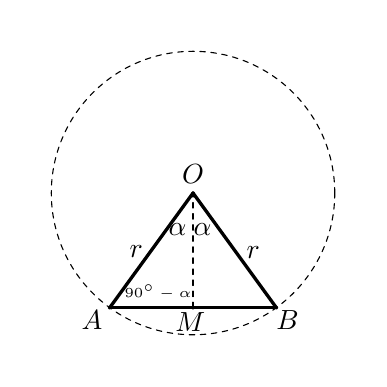
\begin{tikzpicture}[line cap=round,line join=round,x=0.6cm,y=0.6cm]
				\clip(-3.5,-3.5) rectangle (3.5,3.5);
				\draw [line width=0.4pt,dash pattern=on 2pt off 2pt] (0.,0.) circle (3.);
				\draw [line width=1.2pt] (0.,0.)-- (-1.7633557568774196,-2.427050983124842);
				\draw [line width=1.2pt] (-1.7633557568774196,-2.427050983124842)-- (1.7633557568774187,-2.427050983124843);
				\draw [line width=1.2pt] (1.7633557568774187,-2.427050983124843)-- (0.,0.);
				\draw [line width=0.4pt,dash pattern=on 2pt off 2pt] (0.,-2.4270509831248424)-- (0.,0.);
				\draw (-0.72113564155812,-0.44860212696045376) node[anchor=north west] {$\alpha$};
				\draw (-0.194539074291020643,-0.44860212696045376) node[anchor=north west] {$\alpha$};
				\draw (-1.5514237951230748,-0.9125662957500137) node[anchor=north west] {$r$};
				\draw (0.9260216617656386,-0.9351986942275532) node[anchor=north west] {$r$};
				\draw (-1.6569611745698583,-1.7423404264780615) node[anchor=north west] {{\tiny $90^\circ-\alpha$}};
				\draw [fill=black] (0.,0.) circle (0.5pt);
				\draw[color=black] (-0.0019066758134811332,0.394454716327893) node {$O$};
				\draw [fill=black] (-1.7633557568774196,-2.427050983124842) circle (0.5pt);
				\draw[color=black] (-2.1406683319409643,-2.6882866796624014) node {$A$};
				\draw [fill=black] (1.7633557568774187,-2.427050983124843) circle (0.5pt);
				\draw[color=black] (2.001060589448765,-2.6882866796624014) node {$B$};
				\draw [fill=black] (0.,-2.4270509831248424) circle (0.5pt);
				\draw[color=black] (-0.058487672007329905,-2.7282866796624014) node {$M$};
			\end{tikzpicture}
		\end{figure}
	\end{columns}
\end{frame}

\begin{frame}
	至此, 我们已经给出了$S_n$的一般公式. 不过, 研究这个公式的增减性已经超出了我们目前的能力范围.\par
	我们回到书中的数据, 即$C=20$, 分别求出$S_4$, $S_6$, $S_8$, $S_{12}$, $S_\infty$(可以简单地理解为圆).
	轻易计算可以得出
	\[S_4=25, S_6=\frac{50\sqrt{3}}{3}=28.8675\cdots,S_8=\frac{25(1+\sqrt{2})}{2}=30.1777\cdots,\]
	\[S_{12}=\frac{50+25\sqrt{3}}{3}=31.1004\cdots, S_\infty=\frac{100}{\mathrm{\pi}}=31.8310\cdots.\]
	可见, 当$n$增加时, $S_n$也在不断地增加, 直到趋于$100/\mathrm{\pi}$.
\end{frame}

\end{document}